\chapter{平面电磁波与偏振}\label{ch:b2:plane-waves-polarization}

戴着偏光太阳镜歪一歪头，湿路面上的眩光
便时隐时现；把眼镜转到手机屏幕前，
屏幕便一片漆黑。到达你眼睛的光不只是
具有频率和强度的波：它还有一个\emph{振动方向
}，每一块偏振片、屏幕、立体电影镜片和光纤连接器都与它打交道。
本章求解真空中的麦克斯韦方程组——
即横向电场与磁场互相垂直的平面波——
考察这些波所覆盖的光谱，
并研究偏振：如何描述它，
如何用偏振片选取它（马吕斯定律），
以及如何用双折射片改变它。

\section{真空中的平面波}

\begin{theorem}[波动方程；平面行进谐波]\label{thm:b2:plane-waves-polarization:wave}
\index{电磁波}\index{平面波（电磁）}\index{横向性}
在无电荷、无电流的真空中，麦克斯韦方程组给出
\[
\Delta\vect E = \frac1{c^2}\frac{\partial^2\vect E}{\partial t^2} , \qquad
\Delta\vect B = \frac1{c^2}\frac{\partial^2\vect B}{\partial t^2} , \qquad
c = \frac1{\sqrt{\varepsilon_0\mu_0}} = \qty{2.998e8}{m/s} .
\]
\emph{平面行进谐波}（PPH 波）$\underline{\vect E} =
\underline{\vect E}_0\,\eu^{\iu(\omega t - \vect k\cdot\vect r)}$ 是一个解，前提是
$\omega = ck$（无色散），此时麦克斯韦方程组要求
\[
\vect k\cdot\vect E = 0 , \qquad
\vect B = \frac{\vect k\wedge\vect E}\omega = \frac{\vect u\wedge\vect E}c ,
\]
其中 $\vect u = \vect k/k$ 为传播方向，该波为
\emph{横波}，$(\vect E, \vect B, \vect u)$ 构成右手正交标架，
$\vect E$ 与 $\vect B$ 同相，且 $B = E/c$。其强度为
$I = \varepsilon_0cE_0^2/2$，并携带动量流 $I/c$
（见\cref{ch:b2:poynting-vector}）。
\end{theorem}

\begin{proof}
波动方程的推导见\cref{exo:b2:maxwell-equations:11}。
对 $\eu^{\iu(\omega t - \vect k\cdot\vect r)}$，$\partial_t \to \iu\omega$，$\vect\nabla \to
-\iu\vect k$：$\Delta \to -k^2$，故 $k^2 = \omega^2/c^2$；麦克斯韦--高斯定律给出 $-\iu
\vect k\cdot\underline{\vect E} = 0$，麦克斯韦--磁高斯定律给出 $\vect k\cdot\underline{\vect B} = 0$，
麦克斯韦–法拉第定律给出 $-\iu\vect k\wedge\underline{\vect E} = -\iu\omega\underline{\vect B}$，由此
$\underline{\vect B} = \vect k\wedge\underline{\vect E}/\omega$，其模为 $kE/\omega = E/c$，且
与二者都垂直；麦克斯韦–安培定律此时自动满足。
\end{proof}

\begin{omfigure}
\begin{tikzpicture}[font=\small, x=1cm, y=1cm, >=Stealth]
  \draw[->, thick] (-0.3,0) -- (7.4,0) node[right, font=\footnotesize] {$\vect u$};
  \draw[omDef, thick, domain=0:6.8, samples=80] plot (\x,{1.1*cos(deg(1.2*\x))});
  \draw[omProp, thick, domain=0:6.8, samples=80] plot (\x,{-0.4*cos(deg(1.2*\x))});
  \foreach \x in {0,0.65,...,6.6} {
    \pgfmathsetmacro{\e}{1.1*cos(deg(1.2*\x))}
    \draw[omDef, ->] (\x,0) -- (\x,\e);
    \draw[omProp, ->] (\x,0) -- ({\x+0.55*\e*0.36},{-0.4*\e*0.9});
  }
  \node[omDef, font=\footnotesize] at (0.4,1.45) {$\vect E$}; \node[omProp, font=\footnotesize] at (0.9,-0.75) {$\vect B = \vect u\wedge\vect E/c$};
  \draw[<->] (0,-1.3) -- (5.24,-1.3) node[midway, below, font=\footnotesize] {$\lambda = 2\pi/k = c/f$};
\end{tikzpicture}

{\small 某一时刻的平面行进谐波：$\vect E$ 与
$\vect B$ 彼此垂直，并都垂直于传播方向，同相，
$B = E/c$；整个图样沿 $\vect u$ 方向以 $c$ 平移。}
\end{omfigure}

\begin{remark}[光谱]\label{rem:b2:plane-waves-polarization:spectrum}
\index{电磁波谱}
一个方程，一个速率，频率跨越二十个数量级。
无线电波：\qty{30}{kHz}--\qty{300}{MHz}（$\lambda$ 从 \qty{10}{km} 到 \qty{1}{m}），
用于天线与电路（见\cref{ch:b2:dipole-radiation}）。微波：
\qty{300}{MHz}--\qty{300}{GHz}，用于雷达、微波炉、移动电话以及宇宙
背景辐射。红外线：直至 \qty{400}{THz}（\qty{750}{nm}），是我们周围一切物体的热
辐射（见\cref{ch:b2:thermal-radiation}）。
可见光：\qty{400}{THz}--\qty{750}{THz}，从 \qty{750}{nm}（红）到 \qty{400}{nm}
（紫）——跨越一个倍频程，光子能量为 $1.6$ 到 \qty{3.1}{eV}。紫外线直至
\qty{10}{nm}；X 射线直至 \qty{10}{pm}（\qty{100}{keV}），来自原子内层壳层
与制动电子；更高频率的伽马射线来自原子核。只有波源
与探测器不同：波本身是相同的。
\end{remark}

\begin{omfigure}
\begin{tikzpicture}[font=\small, x=1cm, y=1cm, >=Stealth]
  \draw[->, thick] (0,0) -- (13.2,0) node[right, font=\footnotesize] {$f$};
  \foreach \x/\l in {0/$10^4$, 2/$10^6$, 4/$10^8$, 6/$10^{10}$, 8/$10^{12}$, 10/$10^{14}$, 12/$10^{16}$} {
    \draw (\x,-0.1) -- (\x,0.1); \node[font=\scriptsize, below] at (\x,-0.12) {\l};
  }
  \node[font=\scriptsize, below] at (13.0,-0.12) {Hz};
  \fill[omDef!30] (0,0.3) rectangle (4.5,1.0); \node[font=\footnotesize] at (2.25,0.65) {无线电};
  \fill[omDef!50] (4.5,0.3) rectangle (7.5,1.0); \node[font=\footnotesize] at (6.0,0.65) {微波};
  \fill[omThm!30] (7.5,0.3) rectangle (10.6,1.0); \node[font=\footnotesize] at (9.05,0.65) {红外};
  \fill[omProp!60] (10.6,0.3) rectangle (10.9,1.0);
  \fill[omThm!60] (10.9,0.3) rectangle (12.5,1.0); \node[font=\footnotesize] at (11.7,0.65) {紫外};
  \fill[omExo!50] (12.5,0.3) rectangle (13.2,1.0); \node[font=\footnotesize] at (12.85,0.65) {X、$\gamma$};
  \node[font=\scriptsize, omProp] at (10.75,1.3) {可见光};
  \node[font=\scriptsize] at (1.0,1.45) {$\lambda = \qty{30}{km}$}; \node[font=\scriptsize] at (6.0,1.45) {\qty{3}{cm}}; \node[font=\scriptsize] at (10.75,1.75) {\qty{600}{nm}}; \node[font=\scriptsize] at (12.5,1.45) {\qty{10}{nm}};
\end{tikzpicture}

{\small 按对数频率标度画出的电磁波谱；
可见光波段只是一条细缝——二十个数量级中的一个倍频程。}
\end{omfigure}

\section{偏振}

\begin{definition}[偏振态]\label{def:b2:plane-waves-polarization:states}
\index{偏振（光）}\index{线偏振}\index{圆偏振}\index{椭圆偏振}\index{自然光}
对沿 $z$ 方向传播的 PPH 波，在平面 $z = $ 常数上的电场为
\[
\vect E = E_{0x}\cos(\omega t - kz)\,\vect e_x + E_{0y}\cos(\omega t - kz - \varphi)\,\vect e_y ,
\]
一般情况下，$\vect E$ 的端点描出一个椭圆：\emph{椭圆
偏振}。两种特殊情形：$\varphi = 0$ 或 $\pi$ 时，\emph{线偏振}，
电场沿固定方向振动，该方向的倾角为 $\arctan(\pm E_{0y}/E_{0x})$，
自 $x$ 轴量起；$E_{0x} = E_{0y}$ 且 $\varphi = \pm\pi/2$ 时，\emph{圆
偏振}，$\vect E$ 的模保持不变，以 $\omega$ 转动，
按迎着波看去的转向，分为右旋或左旋。
\emph{自然光}（非偏振光）来自灯或太阳，是一连串短的波列，
各列波的偏振方向随机且快速变化：
平均而言，没有任何方向占优。任何偏振
都可以分解为两个线偏振（或两个圆偏振）分量。
\end{definition}

\begin{proof}
记 $X = E_x/E_{0x}$，$Y = E_y/E_{0y}$，则 $X = \cos\theta$，$Y = \cos(\theta - \varphi)$，于是
$X^2 + Y^2 - 2XY\cos\varphi = \sin^2\varphi$，为椭圆，
退化为直线 $Y = \pm X$（$\varphi = 0, \pi$）；当 $E_{0x} = E_{0y}$ 时，
$\varphi = \pm\pi/2$ 时则退化为圆。
\end{proof}

\begin{proposition}[起偏器与马吕斯定律]\label{prop:b2:plane-waves-polarization:malus}
\index{起偏器}\index{马吕斯定律}\index{检偏器}
一块\emph{起偏器}透射 $\vect E$ 沿其透射轴 $\vect p$ 的分量，
并吸收其余分量（一片排列整齐的长分子，沿长度方向导电——
透射偏振方向与分子垂直）。
入射的线偏振光（强度为 $I_0$），
其方向与透射轴成夹角 $\theta$，
出射光为 $\vect p$ 方向的分量，沿 $\vect p$ 线偏振，强度为
\[
I = I_0\cos^2\theta \qquad\text{（马吕斯）} ;
\]
自然光出射时强度为 $I_0/2$，且沿 $\vect p$ 偏振。
正交放置的两块起偏器不透光；若在其间
以 \qty{45}{\degree} 插入第三块，则透过 $I_0/8$。
\end{proposition}

\begin{proof}
透射振幅为 $E_0\cos\theta$，且 $I \propto E_0^2$。对自然光，
$\cos^2\theta$ 对全部 $\theta$ 的平均为 $\tfrac12$。三块起偏器：
$\tfrac12\cdot\cos^2 45^\circ\cdot\cos^2 45^\circ = \tfrac18$——中间
起偏器并非仅使光减弱，而是\emph{转动}了偏振方向。
\end{proof}

\begin{omfigure}
\begin{tikzpicture}[font=\small, x=1cm, y=1cm, >=Stealth]
  \begin{scope}
    \draw[->, thick] (-0.4,0) -- (7.2,0) node[right, font=\footnotesize] {$z$};
    \foreach \x/\a/\l in {1.0/90/$\vect p_1$, 3.5/45/$\vect p_2$, 6.0/0/$\vect p_3$} {
      \draw[thick, fill=omExo!15] (\x,0) ellipse (0.35 and 1.1);
      \draw[omThm, very thick, <->] ({\x-0.3*cos(\a)},{-0.9*sin(\a)}) -- ({\x+0.3*cos(\a)},{0.9*sin(\a)});
      \node[omThm, font=\footnotesize] at (\x,1.4) {\l};
    }
    \node[font=\footnotesize] at (2.25,-1.5) {$I_0/2$}; \node[font=\footnotesize] at (4.75,-1.5) {$I_0/4$}; \node[font=\footnotesize] at (6.9,-1.5) {$I_0/8$};
    \node[font=\footnotesize] at (0.2,-1.5) {$I_0$，自然光};
  \end{scope}
  \begin{scope}[xshift=10.2cm]
    \begin{axis}[omaxis, axis x line=bottom, axis y line=left, width=4.6cm, height=3.8cm, at={(0,-1.6cm)},
        xlabel={$\theta$}, ylabel={$I/I_0$}, xmin=0, xmax=180, ymin=0, ymax=1.1, xtick={0,90,180}, xticklabels={$0$, $90^\circ$, $180^\circ$}, ytick={0.5,1}, samples=100,
        xlabel style={at={(axis description cs:1.0,0.0)}, anchor=west},
        ylabel style={at={(axis description cs:-0.12,0.5)}, rotate=90, anchor=south}]
      \addplot[omDef, thick, domain=0:180] {cos(x)^2};
    \end{axis}
  \end{scope}
\end{tikzpicture}

{\small 左：自然光依次通过位于 $0^\circ$、$45^\circ$
和 $90^\circ$ 处的三块起偏器——中间一块使八分之一的光得以通过，
而仅这一对起偏器便会挡住全部光。右：马吕斯定律。}
\end{omfigure}

\begin{example}[太阳镜、屏幕与照片]\label{ex:b2:plane-waves-polarization:uses}
从水面或沥青路面以掠射角反射的光大多
为水平偏振（布儒斯特角，见\cref{ch:b2:wave-interfaces}）：
透射轴为竖直方向的太阳镜可以挡住眩光，保留
其余的光。液晶屏幕发出偏振光，经
与之成 \qty{90}{\degree} 的起偏器后便呈黑色。摄影师的偏振滤光片
会使天空变暗（散射光部分偏振，
见\cref{ch:b2:dipole-radiation}），并消除玻璃上的反光。
\end{example}

\section{双折射与波片}

\begin{proposition}[波片]\label{prop:b2:plane-waves-polarization:plates}
\index{双折射}\index{波片}\index{半波片}\index{四分之一波片}\index{快轴}\index{慢轴}
在\emph{双折射}晶体（方解石、石英、云母；也包括
拉伸的塑料薄片）中，沿给定方向传播的波
分裂为两个线偏振分量，分别沿板的\emph{快轴}和
\emph{慢轴}方向，以不同折射率 $n_f <
n_s$ 传播（在本阶段不加证明地承认——晶体沿各轴的响应不同）。
一块厚度为 $e$ 的波片使慢分量产生的相位延迟为
\[
\delta = \frac{2\pi}\lambda(n_s - n_f)\,e .
\]
一块\emph{半波片}（$\delta = \pi$）使与快轴成
$\alpha$ 角的线偏振变为方向为 $-\alpha$ 的线偏振，它
将其转过 $2\alpha$。一块\emph{四分之一波片}（$\delta = \pi/2$）
使与轴成 \qty{45}{\degree} 的线偏振化为圆偏振光，
圆偏振光则反变为线偏振；在其他角度时，变为
沿波片轴方向的椭圆偏振光。
\end{proposition}

\begin{proof}
设入射场为 $E_0(\cos\alpha\,\vect e_f + \sin\alpha\,\vect e_s)\cos\omega t$；
经波片后为 $E_0[\cos\alpha\cos\omega t\,\vect e_f + \sin\alpha\cos(\omega t - \delta)
\vect e_s]$。当 $\delta = \pi$ 时，$\vect e_s$ 分量变号，方向为
$(\cos\alpha, -\sin\alpha)$。当 $\delta = \pi/2$ 且 $\alpha = 45^\circ$ 时，$(E_0/\sqrt2)(\cos
\omega t, \sin\omega t)$，为圆。
\end{proof}

\begin{omfigure}
\begin{tikzpicture}[font=\small, x=1cm, y=1cm, >=Stealth]
  \begin{scope}
    \draw[->] (-1.5,0) -- (1.5,0) node[right, font=\footnotesize] {$x$}; \draw[->] (0,-1.5) -- (0,1.5) node[above, font=\footnotesize] {$y$};
    \draw[omDef, very thick, <->] (-1.1,-0.8) -- (1.1,0.8); \node[omDef, font=\footnotesize] at (1.25,1.05) {线偏振};
    \node[font=\footnotesize] at (0,-1.9) {$\varphi = 0$};
  \end{scope}
  \begin{scope}[xshift=4.2cm]
    \draw[->] (-1.5,0) -- (1.5,0); \draw[->] (0,-1.5) -- (0,1.5);
    \draw[omDef, very thick, postaction={decorate, decoration={markings, mark=at position 0.3 with {\arrow{>}}}}] (0,0) circle (1.0);
    \node[omDef, font=\footnotesize] at (1.25,1.15) {圆偏振};
    \node[font=\footnotesize] at (0,-1.9) {$E_{0x} = E_{0y}$, $\varphi = \pm\pi/2$};
  \end{scope}
  \begin{scope}[xshift=8.4cm]
    \draw[->] (-1.5,0) -- (1.5,0); \draw[->] (0,-1.5) -- (0,1.5);
    \draw[omDef, very thick, rotate=30, postaction={decorate, decoration={markings, mark=at position 0.3 with {\arrow{>}}}}] (0,0) ellipse (1.2 and 0.55);
    \node[omDef, font=\footnotesize] at (1.3,1.15) {椭圆偏振};
    \node[font=\footnotesize] at (0,-1.9) {一般 $\varphi$};
  \end{scope}
  \begin{scope}[xshift=12.4cm]
    \draw[thick, fill=omExo!15] (0,0) ellipse (0.35 and 1.3);
    \draw[omThm, thick, ->] (0,0) -- (0,1.0) node[right, font=\footnotesize, yshift=-3pt] {慢轴};
    \draw[omThm, thick, ->] (0,0) -- (0.5,0) node[right, font=\footnotesize] {快轴};
    \node[font=\footnotesize] at (0,-1.9) {$\delta = 2\pi(n_s - n_f)e/\lambda$};
  \end{scope}
\end{tikzpicture}

{\small 平面波的偏振态（迎着
入射光观察）以及一块带快轴和慢轴的双折射片。}
\end{omfigure}

\begin{example}[波片的应用]\label{ex:b2:plane-waves-polarization:plateuses}
置于起偏器与反射镜之间的四分之一波片构成
\emph{光隔离器}：光射出时为圆偏振，返回时为
旋向相反的圆偏振光，经波片后变为线偏振光，
其方向与起偏器成 \qty{90}{\degree}，并被吸收——因而
没有任何反射光返回激光器。3D 电影的左右眼图像
以相反的圆偏振投射，并由眼镜中的四分之一波片–起偏器
组合加以分开，这种组合在头部倾斜时依然有效（线偏振起偏器则不行）。
透明尺子置于正交的起偏器之间，
会呈现彩色条纹：应力使塑料产生双折射，
工程师由此可从模型的条纹图样读出
模型中的应力分布。
\end{example}

\begin{method}[沿光学系统追踪偏振]\label{met:b2:plane-waves-polarization:method}
（1）选取坐标轴，将入射场写成两个分量及其
相位差。（2）起偏器：保留其在偏振轴上的投影
（振幅 $\times\cos$，强度 $\times\cos^2$；自然光
$\times\tfrac12$）。（3）波片：分别投影到快轴和慢轴，
将慢轴分量延迟 $\delta$，再合成。（4）读结果：相位为 $0$ 或 $\pi$
时为线偏振，$\pm\pi/2$ 且振幅相等时为圆偏振。
（5）检验未知光束：旋转起偏器（强度有变化则含线偏振或
椭圆偏振成分），再加一块四分之一波片（圆偏振变为
线偏振，可被消光）。
\end{method}

\section{练习}

\begin{exercise}[$\star$]\label{exo:b2:plane-waves-polarization:1}
一座频率为 \qty{100}{MHz} 的调频电台，在接收处的光强为
\qty{1.0}{\micro W/m^2}。求波长、波数、周期；振幅 $E_0$ 与
$B_0$；能量密度；与 $\vect E$ 方向一致放置的 \qty{1}{m} 天线中产生的电动势；
光子通量（每平方米每秒）。
\end{exercise}

\begin{exercise}[$\star$]\label{exo:b2:plane-waves-polarization:2}
求 $\lambda = \qty{1}{km}$、\qty{10}{cm}、
\qty{10}{\micro m}、\qty{550}{nm}、\qty{10}{nm}、\qty{0.1}{nm}、\qty{1}{pm} 时的频率与光子能量（以 eV 为单位），并说出每种波长所属的
波段；求 \qty{1}{MeV} 伽马射线的波长，以及
\qty{2.7}{K} 宇宙背景辐射（峰值约在 \qty{160}{GHz}）的波长。
\end{exercise}

\begin{exercise}[$\star$]\label{exo:b2:plane-waves-polarization:3}
光强为 $I_0$ 的线偏振光射到一个起偏器上，该起偏器与入射光偏振方向成
\qty{30}{\degree}，然后射到与第一个成 \qty{60}{\degree} 的第二个起偏器上，再射到与第一个成
\qty{90}{\degree} 的第三个起偏器上：求经过每个起偏器后的光强。
若入射为自然光，结果如何？若去掉中间那个起偏器，结果有何变化？
\end{exercise}

\begin{exercise}[$\star$]\label{exo:b2:plane-waves-polarization:4}
验证 $\vect E = E_0\cos(\omega t - kz)\,\vect e_x$，$\vect B = (E_0/c)\cos(\omega t
- kz)\,\vect e_y$ 在 $\omega =
kc$ 时满足真空中的四个麦克斯韦方程，哪一个方程决定 $\vect B$ 的方向，哪一个决定其
大小？若试取 $\vect E$ 沿 $\vect e_z$ 方向，会出现什么情况？
\end{exercise}

\begin{exercise}[$\star\star$]\label{exo:b2:plane-waves-polarization:5}
\emph{圆偏振光。}（a）写出沿 $z$ 方向传播的
圆偏振波的电场，并证明 $|\vect E|$ 为常量，而其方向
以角频率 $\omega$ 旋转。（b）证明两个振幅相等、旋向相反的
圆偏振波之和为线偏振波，其偏振方向由二者的
相对相位决定。（c）圆偏振光通过起偏器后会得到什么结果？
光强是否依赖于起偏器的角度？（d）那么如何
区分圆偏振光与自然光？
\end{exercise}

\begin{exercise}[$\star\star$]\label{exo:b2:plane-waves-polarization:6}
石英在 \qty{589}{nm} 处有 $n_s - n_f = 0.0091$。（a）求最低阶的
四分之一波片的厚度，以及半波片的厚度。（b）对于 \qty{589}{nm} 设计的
四分之一波片，若用于 \qty{450}{nm}，求其相位延迟
（忽略折射率随波长的变化）；对于与快轴成 \qty{45}{\degree} 的
线偏振光，出射光是什么？（c）为什么厚度为 $e +
m\lambda/(n_s - n_f)$ 的“多级”波片对波长与温度更敏感？（d）为什么
波片的厚度必须控制在优于一微米的精度内？
\end{exercise}

\begin{exercise}[$\star\star$]\label{exo:b2:plane-waves-polarization:7}
半波片。（a）证明：与快轴成 $\alpha$ 角的线偏振光出射后为
与快轴成 $-\alpha$ 角的线偏振光。（b）由此可知，将波片旋转 $\beta$
会使偏振方向旋转 $2\beta$：要使竖直偏振变为水平偏振，
波片应旋转多大角度？（c）半波片对圆偏振光有何作用？
（d）将半波片置于正交的两个起偏器之间并缓慢转动，
请画出透射光强随其角度变化的示意图。
\end{exercise}

\begin{exercise}[$\star\star$]\label{exo:b2:plane-waves-polarization:8}
将 $N$ 个起偏器依次排列，每个相对于前一个旋转
$\pi/2N$，最后一个与第一个成 \qty{90}{\degree}。对于与第一个
起偏器方向一致的线偏振光，求其在 $N = 1, 2, 5, 10, 100$ 时的透过率；
并求 $N \to \infty$ 时的极限（可用 $\cos^{2N}(\pi/2N) \approx
1 - \pi^2/4N$）。评述：偏振方向可以无损失地转过 \qty{90}{\degree}，
这是靠什么实现的？
\end{exercise}

\begin{exercise}[$\star\star$]\label{exo:b2:plane-waves-polarization:9}
\emph{部分偏振。}对一束光前置一个旋转的起偏器，
测得最大光强为 $I_{\max}$，最小光强为 $I_{\min}$。（a）将该光束视为自然光 $I_n$
与线偏振光 $I_p$ 之和，用它们表示 $I_{\max}$ 与
$I_{\min}$，并求偏振度 $p = I_p/(I_n + I_p) =
(I_{\max} - I_{\min})/(I_{\max} + I_{\min})$。（b）晴朗天空中与太阳成 \qty{90}{\degree} 方向的光，
$I_{\max}/I_{\min} = 5$，求 $p$。（c）湖面在接近布儒斯特角处反射的光，$p = 0.9$，
偏振太阳镜最多能滤除多少？（d）仅用一个起偏器，
能否区分部分线偏振光与部分圆偏振光？
还需要什么？
\end{exercise}

\begin{exercise}[$\star\star\star$]\label{exo:b2:plane-waves-polarization:10}
\emph{两束交叉光束。}两列振幅与频率相同的 PPH 波，
均沿 $\vect e_y$ 方向偏振，在 $xz$ 平面内传播，
分别以 $\pm\theta$ 角（相对 $z$ 轴）传播。（a）写出总场，并证明它是一列
沿 $z$ 方向传播的波，其振幅沿 $x$ 方向按 $\cos(kx\sin\theta)$ 调制。
（b）求暗面（即干涉条纹）的间距；
分别计算 $\lambda = \qty{633}{nm}$、$\theta = \qty{5}{\degree}$ 时的数值，以及
$\theta = \qty{90}{\degree}$（反向传播）时的数值。（c）求图样沿 $z$ 方向的相速度，
并与 $c$ 比较，是否有东西的传播速度快于
光速？（d）求坡印廷矢量的时间平均值，并证明其
$x$ 分量为零：能量沿 $z$ 方向在亮
面中流动。
\end{exercise}

\begin{exercise}[$\star\star\star$]\label{exo:b2:plane-waves-polarization:11}
\emph{液晶像素。}一个扭曲向列型液晶盒置于正交起偏器之间，
在不加电压时使光的偏振方向旋转 \qty{90}{\degree}，
此时分子取向沿盒内扭转（偏振方向随之转动，
在本阶段不加证明地承认），而当几伏电压使其解扭时，偏振方向完全不再旋转。
（a）比较两种状态的透射：哪一种是亮态？
（b）实际液晶盒在设计波长下旋转 $90^\circ \pm 5^\circ$，
求对比度 $I_{\text{亮}}/I_{\text{暗}}$，设暗态因残余
\qty{5}{\degree} 误差而漏光。（c）为何按 \qty{550}{nm} 设计的
液晶盒在暗态下仍会漏出部分蓝光和红光？
（可将旋转视为许多薄的类半波
延迟器的叠加。）（d）彩色像素由三个此类液晶盒配合滤光片组成，为何
屏幕透过某一角度的起偏器看去会变黑，
该角度说明了什么？
\end{exercise}

\begin{exercise}[$\star\star\star$]\label{exo:b2:plane-waves-polarization:12}
\emph{旋光性。}在糖溶液中，两种圆偏振分量以略有不同的折射率
$n_L$ 与 $n_R$ 传播。（a）将线偏振光分解为圆偏振分量，证明
经过长度 $\ell$ 后偏振仍为线偏振，但方向转过了
$\theta = \pi(n_L - n_R)\ell/\lambda$。（b）一根 \qty{1}{dm} 长的管中盛有
\qty{0.10}{g/mL} 的蔗糖溶液，使钠光旋转 \qty{6.65}{\degree}，
求 $n_L - n_R$。（c）用旋光计测量 $\theta$，精度为 \qty{0.01}{\degree}，
求浓度的精度。（d）同样的效应可在玻璃中由沿光束方向的磁场产生，
即法拉第效应，$\theta = VB\ell$，其中 $V \approx
\qty{4}{rad.T^{-1}.m^{-1}}$）：为何法拉第旋转器与糖管不同，
光沿原路返回时，
其旋转不会抵消，
这如何使其成为隔离器？
\end{exercise}

\begin{omfigure}
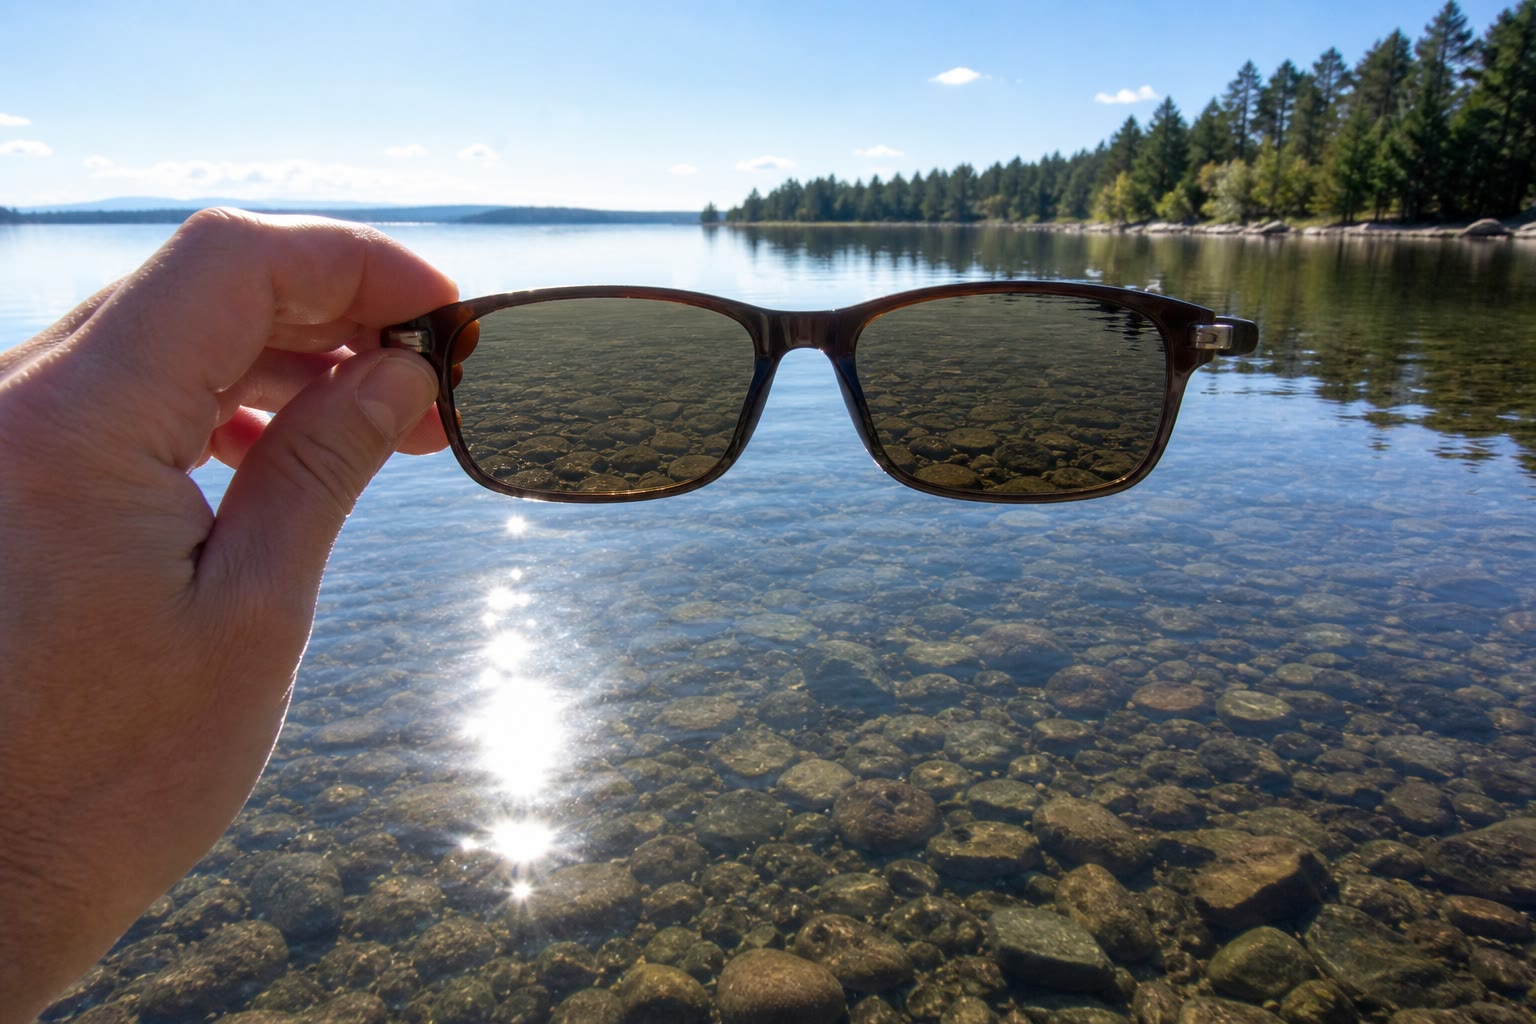
\includegraphics[width=0.58\linewidth]{images/book4/ai/b4-13-polarizing-sunglasses-lake.jpg}

{\small 手持偏振太阳镜对着湖面：布儒斯特角附近反射的眩光为水平偏振，被镜片的竖直透振轴挡住，湖底因此得以显现。}
\end{omfigure}

\section{问题：波、屏幕与帆}

\begin{problem}[{周末问题——将激光束拆解为其场，
一块以偏振“作画”的屏幕，以及一艘
借光航行的航天器}]
\label{pb:b2:plane-waves-polarization:1}

\medskip
\noindent\textbf{第一部分——光束。}
一台氦氖激光器发出 \qty{10}{mW}、波长为 \qty{632.8}{nm} 的光，光束
直径为 \qty{1.0}{mm}，沿 $x$ 方向线偏振，沿
$z$ 方向传播。
\begin{enumerate}
  \item 求频率、波数与光子能量，以及
        每秒发出的光子数。
  \item 求强度、振幅 $E_0$ 与 $B_0$，并写出 $\vect E(z, t)$ 和
        $\vect B(z, t)$。
  \item 求能量密度（平均值）以及 \qty{1}{m} 长光束中所含的能量，
        光束在 \qty{1}{ns} 内发出的长度是多少，其中包含
        多少个波长？
  \item 求坡印廷矢量的平均值及其振荡，以及每秒携带的
        动量；求黑色靶与镜子所受的力。
  \item 将 $E_0$ 与束缚氢原子中电子的场比较，
        即 \qty{5e11}{V/m}；将 $B_0$ 与地球磁场
        （\qty{50}{\micro T}）比较。
  \item 求黑色光束挡板上的辐射压强，单位为帕斯卡。
  \item 将一个自由电子置于光束中，求其速度振荡的振幅，
        即电场中的振荡（先忽略磁力）；
        再求其所受磁力与电力之比——为何
        普通光中磁力对物质可以忽略不计，
        原因何在？
  \item 若该光束为圆偏振，写出其场，
        并说明强度与坡印廷矢量有何变化，
        及其随时间的变化如何？
  \item 光束先通过透振轴与 $x$ 轴成
        \qty{30}{\degree} 的起偏器，求透射功率；
        再通过与第一个正交的第二个起偏器，求功率；
        若在两者之间插入第三个起偏器，其与第一个成 \qty{45}{\degree}，求功率。
\end{enumerate}

\medskip
\noindent\textbf{第二部分——屏幕。}
一块液晶屏依次为背光（自然光）、一个起偏器、液晶盒，
以及与之正交的起偏器。不加电压时，液晶盒使偏振方向旋转
\qty{90}{\degree}；加电压时则不起作用。
\begin{enumerate}[resume]
  \item 求亮态下透过的背光强度所占比例
        （设起偏器理想），以及暗态下的比例。
  \item 施加某一中间电压时，液晶盒作为延迟器，两轴间相位差为 $\delta$，
        其两轴与起偏器成 \qty{45}{\degree} 角，
        不发生旋转；证明其透射率为
        $\sin^2(\delta/2)$——即灰阶。
  \item 若透过一个相对屏幕输出起偏器转过 \qty{90}{\degree} 的起偏器观察，
        会看到什么？在 \qty{45}{\degree} 时又如何？
  \item 在屏幕上贴一块四分之一波片，使其与起偏器成 \qty{45}{\degree}，
        使输出变为圆偏振：对戴偏振太阳镜的
        观众有何优势？
  \item 若起偏器理想，亮态下将透过背光的一半；
        实际偏振片各自透过理想值的 $85\%$，而
        像素的彩色滤光片透过三分之一的光：
        求白色时到达观众的背光功率比例；
        指出损失大部分光的两个位置。
  \item 实际正交的偏振片漏过 $0.1\%$ 的光：
        求暗室中屏幕的对比度（亮态与暗态之比）。
  \item 摄影师所谓的“圆偏振镜”由一块线偏振起偏器
        与一块成 \qty{45}{\degree} 的四分之一波片组成：相机接收到的是什么，
        以及为何它对其自动对焦中偏振敏感的分束器
        比线偏振光更有利，
        原因何在？
  \item 为何 3D 影院眼镜采用圆偏振而非
        线偏振？两眼之间的串扰将如何变化？
        若观众将头部倾斜 \qty{20}{\degree}，改用线偏振眼镜，
        光强将漏入错误的眼睛（即串扰增大）？
\end{enumerate}

\medskip
\noindent\textbf{第三部分——太阳帆。}
一面面积为 $S = \qty{1000}{m^2}$、总质量为 $m = \qty{50}{kg}$ 的太阳帆，
表面完全反射，位于距太阳 $D = \qty{1.0}{au} = \qty{1.5e11}{m}$ 处
（$I = \qty{1.36}{kW/m^2}$；该处太阳引力为 \qty{5.9e-3}{m/s^2}）。
\begin{enumerate}[resume]
  \item 帆正对太阳时的辐射力；加速度；
        其与太阳引力之比。
  \item 帆与正对太阳的方向成 $\theta$ 角倾斜，证明该力
        垂直于帆面，且与 $\cos^2\theta$ 成正比
        （截获功率 $\times\cos\theta$，沿
        法线方向的动量变化 $\times\cos\theta$）。
  \item 为使帆向外螺旋运动，帆需保持一个沿其
        轨道速度方向的力分量：当 $\theta = \qty{35}{\degree}$ 时，
        求切向加速度；每年获得的速率增量；并与地球的轨道速率
        （\qty{30}{km/s}）作比较。
  \item 同一面帆靠近水星（$D = \qty{0.39}{au}$）时受力为
        $6.6$ 倍，为何其与引力之比
        保持不变？
  \item 该帆膜为 \qty{2}{\micro m} 厚的镀铝塑料：
        若其吸收 $10\%$，并作为黑体从两面辐射，求其在阳光下的温度
        （$\sigma = \qty{5.67e-8}{W.m^{-2}.K^{-4}}$）。
  \item 正对太阳时，帆速增至 \qty{1}{km/s} 所需的时间；
        同样大小的吸收型（黑色）帆能达到什么速率？
  \item 用光子检验光的动量：每秒打在帆上的光子数
        （平均能量为 \qty{2}{eV}）及每个光子的动量
        $hf/c$；由此复算该力。
  \item 小结：光波携带的三个量（能量、
        动量、偏振）以及本题中
        利用各量的装置。
\end{enumerate}
\end{problem}
